\documentclass{standalone}
\usepackage[utf8]{inputenc}
\usepackage{pgf,tikz}
\usepackage{mathrsfs}
\usetikzlibrary{arrows}
\usetikzlibrary{arrows.meta}
\pagestyle{empty}
\begin{document}
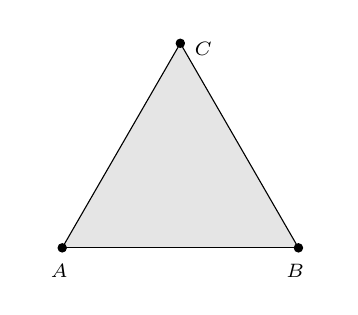
\begin{tikzpicture}[line cap=round,line join=round,>={Stealth},x=3.0cm,y=3.0cm]
\clip(-0.14623591073873005,-0.16475768366802676) rectangle (1.131007128538445,0.9320837963892064);
\fill[line width=0.4pt,fill=black,fill opacity=0.10000000149011612] (0.,0.) -- (1.,0.) -- (0.5,0.8660254037844388) -- cycle;
\draw [line width=0.4pt] (0.,0.)-- (1.,0.);
\draw [line width=0.4pt] (1.,0.)-- (0.5,0.8660254037844388);
\draw [line width=0.4pt] (0.5,0.8660254037844388)-- (0.,0.);
\begin{scriptsize}
\draw [fill=black] (0.,0.) circle (1.5pt);
\draw[color=black] (-0.012738756915974453,-0.09800910675664909) node {$A$};
\draw [fill=black] (1.,0.) circle (1.5pt);
\draw[color=black] (0.986685881162493,-0.09800910675664909) node {$B$};
\draw [fill=black] (0.5,0.8660254037844388) circle (1.5pt);
\draw[color=black] (0.5970185132474226,0.8436870323714358) node {$C$};
\end{scriptsize}
\end{tikzpicture}
\end{document}